\documentclass[14pt,a4paper,titlepage]{report}
\usepackage[utf8]{inputenc}     % accents dans la source
\usepackage[T1]{fontenc}        % nouvelle norme latex
\usepackage[normalem]{ulem}     % 
\usepackage[french]{babel}      % supporter le français
\usepackage{verbatim}           % coder en VERBATIM
\usepackage{moreverb}                   % coder en VERBATIM
\usepackage[pdftex]{graphicx, color}
\graphicspath{{figs/}}
\DeclareGraphicsExtensions{.jpg,.png}
\usepackage{url}                %
\usepackage{float}
\usepackage{hyperref}           % utiliser les liens hypertextes
\usepackage{color}              % utiliser les couleur 
\usepackage{pifont}             % des symboles et des figures
\usepackage{fancybox}           % carrés 
\usepackage[a4paper,
  rmargin=2cm,
  lmargin=2cm,
  tmargin=2cm,
  bmargin=2cm]{geometry}  % mise en page 
\usepackage{listings}           % du code dans latex
\usepackage{fancyhdr}
\usepackage{bibunits}



\begin{document}
\begin{titlepage}
  \begin{flushleft}
    \vspace{3mm}
    
\includegraphics[width=3cm]{upmclogo_m.png}\\
  \end{flushleft}
  \vfil
  \vfil
  \begin{center}
    \Huge\textbf{{PPAR}}\\
    \hrulefill\\
    \Huge\textit{{Probleme des N-CORPS}}\\
  \end{center}
  \hrulefill\\
  \vfil
  \noindent \textbf{ALAHYANE} \bsc{Rachid}
  \hfill 
  \href{mailto:rachid.alahyane@etu.upmc.fr}{rachid.alahyane@etu.upmc.fr}\\ 
  \textbf{CASTELLANOS} \bsc{Cuauhtemoc}
  \hfill 
  \href{mailto:cuauhtemoc.castellanos@etu.upmc.fr}{cuauhtemoc.castellanos@etu.upmc.fr}\\
  \vfil
  \begin{center}	
    \shadowbox{\footnotesize{\emph{PPAR 2009 - \today}}}
  \end{center}
\end{titlepage}





\lhead{PPAR 2009}
\rhead{Probleme des N-corps}
\renewcommand\headrulewidth{2pt}

\newpage
\pagestyle{empty}
\tableofcontents

\newpage
\chapter{Introduction}
\thispagestyle{fancy}
\section{Contexte et objectifs}
\par Dans le cadre du module de programmation parallèle (PPAR)
du Master 2 systèmes et applications répartis (SAR), nous devons réaliser
la parallélisation d'un programme permettant de modéliser la dynamique des galaxies.
Ce problème d'astrophysique appelé aussi le problème des N-corps consiste à 
simuler les interactions dans un espace en 3 dimensions de N corps les uns avec
les autres.\\
\par Dans un premier temps, nous allons paralléliser le code séquentiel de manière 
à le rendre exécutable sur un petit cluster de machines de l'ARI. Pour cela nous 
utiliserons la bibliothèque MPI qui permet facilement de répartir les calculs sur 
plusieurs machines. Nous définirons le stockage en mémoire, l'architecture des
communications entre chaque machines ; nous recouvrirons également les temps de 
communication par le calcul et nous rendrons les communications persistantes.\\
\par Une fois cela effectué, nous utiliserons le fait que chaque noeud (machine)
possède un processeur multi-coeur, nous mettrons en place une parellélisation hybride
multi-processus/multi-threads en utilisant l'API OpenMP.\\
\par En fin, une étude comparative des performances sera fournie,
développant et expliquant les différents résultats des performances obtenues.\\



\chapter{Etat de l'art}
\thispagestyle{fancy}
\par Comme nous allons paralléliser un code séquentiel existant,
nous sommes dépendant du langage de ce code. Le code source fourni 
étant du C, naturellement nous nous dirigerons vers une solution 
de parallélisation MPI/C, que nous avons eu l'occasion de prendre 
en main dans le cadre du module PPAR. Cependant, il reste le choix de la 
version MPI que nous utiliserons.\\

\par La version 1.3 nous fournissait une API permettant d'abstraire 
l'architecture des noeuds et de communiquer avec sans se soucier du réseau. C'est
celle que nous avons utilisé durant les travaux pratiques.\\

\par La version 2.x effectue les mêmes opérations que la version 1.3,
cependant elle permet de gérer un pool de threads et d'effectuer des communications unilatérales.\\

\par Afin de paralléliser le code sur chaque noeud en utilisant des threads,
deux choix s'offrent à nous : utiliser l'API POSIX ou l'API OpenMP.\\
La première est complètement gérée à partir de MPI-2.x mais nous serons sans doute
obligés d'utiliser des verrous pour l'accès aux données partagées par les threads.
Alors que la seconde nous abstrait de ce genre de considérations, en permettant 
des déclarations de variables privées, visibles uniquement pour le thread dans lequel elle est déclarée, 
ou publique visible pour tous les threads.\\

\par Nous utiliserons donc l'API OpenMP.\\

\par Le $"cluster"$ que nous utiliserons pour effectuer nos tests 
est homogène, chaque machine a les mêmes processeurs (la même fréquence et le même nombre de core),
la même quantité de mémoire, et les temps de communications seront sensiblement 
les mêmes entre chaque noeud. Nous effectuerons nos tests dans une des salles 
de l'ARI, les machines étant reliées entre elles par un réseau local nous considèrerons 
les canaux comme fiables et MPI nous en garantie le caractère FIFO.
De plus, comme nous comptons recouvrir les temps
de communications par le calcul et que nous allons utiliser l'API OpenMP 
pour créer des threads, nous n'utiliserons pas les nouvelles fonctionnalités offertes
par MPI-2.x. Nous utiliserons donc la version 1.3 de MPI.\\

\par Il reste cependant un point important à clarifiées. Nous sommes dans un environnement particulier ; 
celui fournis par l'ARI ; où notre compte utilisateur est stocké sur un NFS, un système de fichier 
distribué qui nous garantie le fait de pouvoir se logger sur n'importe quelle machine du réseau 
de l'ARI. En utilisant le fait que nous pouvons accéder à n'importe quel fichier présent sur 
notre session et développer ainsi un programme parallèle à pseudo mémoire partagée.
Ainsi lors de l'initialisation du système, chaque noeud  pourrait aller lire dans le fichier 
que dont l'on souhaite calculer les interactions et ainsi éviter les appels à la fonction 
MPI\_Scatter() qui permet d'initialiser chaque noeud du système avec les corps qu'il va héberger.\\

\par Cependant, ne connaissant pas l'environnement sur lequel les correcteurs exécuterons notre 
programme nous avons fait le choix d'utiliser l'initialisation par appel à la fonction MPI\_Scatter().\\

\par De plus nous pourrions utiliser des fichiers afin de communiquer entre chaque noeud, mais le NFS ne nous
donne que l'illusion du système de fichier local, donc il y aurait quand même deux accès réseau pour 
transférer les données, et il faudrait en plus compter deux accès disque, l'un en écriture, l'autre en lecture.
Ce qui est long par rapport à une émission et réception de message MPI.\\



\chapter{Architectures et réalisation en MPI}
\thispagestyle{fancy}
\section{Parallèlisation}

\par Dans un premier temps il est necessaire de trouver les points de parallèlisation 
du programme séquentiel. Pour ce faire il est nécessaire de bien connaitre l'algorithme 
utilisé.\\
\par L'algorithme séquentiel consiste à stocker les corps dans un tableau de structures ou une structure 
de tableaux (selon si la constante \_BODIES\_SPLIT\_DATA\_ est définies ou pas), à parcourir 
cette structure et à calculer une à une les interactions entre deux corps, puis à les déplacer.\\

\par L'interet de la parallèlisation est de pouvoir répartir la structure de donnée sur tout les
noeuds du système afin d'alléger la mémoire utilisée par chaque noeud, et ainsi augmenter le 
nombre de corps de la simulation.\\

\par Une fois ceci fait il faut que malgrés la séparation des données nous réussissions a calculer
les interactions entre chaque corps. Nous pouvons décidé d'utiliser une architecture centralisée 
ou distribuée, sachant que nous devons effectuer une sauvegarde à chaque pas de temps ($dt$) si l'option 
d'éxécution --save est présente en entrée.\\

\subsection{Solution centralisée}
\par L'avantage de la solution centralisée, c'est qu'un processus (maître) distribue le travail aux autres
(les esclaves). Ainsi cela permet de distribuer plus de travail aux noeuds plus puissants et moins aux
plus lents. Ce qui dans notre cas, ne nous concerne pas étant donné que les noeuds sont considérés homogènes
(ils sont tous de même puissance).\\

\par L 'inconvénient est que cette solution fonctionne trés bien avec un petit nombre de noeuds 
mais elle ne tient pas le passage à l'échelle (si on augmente le nombre de machine 
de manière consécante).\\

\par Cependant pour effectuer les sauvegardes de chaque pas de temps ($dt$) ce sera la solution a adoptée. 
Toutes les valeurs calculées seront rapatriées vers le processus 0 qui se chargera d'effectuer 
l'écriture  dans le fichier cible.\\

\par De même pour verifierque la somme des forces est nulle on effectuera des sommes partielle
sur chaque noeud, puis on fera leur somme sur le processus de rang 0.\\

\subsection{Solution distribuée}
\par La solution distribuée passe trés bien à l'échelle, mais il est difficile de
la rendre adaptable dynamiquement et s'utilise de préférence dans une architecture homogène
( où les temps de calcule sont sensiblement les mêmes).\\

\par C'est ainsi que fonctionnera le calcul des interactions des corps. Au temps $t=0$, chaque noeud 
calcule les interactions entre les corps dont il dispose localement. Au temps $t=0+dt$ chaque
processus envoie aux autres noeuds les données qu'il a calculé et reçoit les données d'un corps
calculées d'un autre noeud. On réitère cette operation $p-2$ fois ainsi chaque processus a
calculé les interactions avec tout les corps du système.\\

\section{Structures}

\par Le programme séquentiel nous donne le choix de la représentation en mémoires des 
corps. Si la macro \_BODIES\_SPLIT\_DATA\_ est définie, les corps sont stockés soit
dans une structure de tableaux, soit dans un tableau de structures.\\


\subsection{Tableau de structures}

\par Le fait d'utiliser un tableau de structure fera qu'à l'initisation, au lieu de faire huit 
MPI\_scatter() (un pour chaque champs dans le cas de strucures de tableaux) on en fera qu'un seul.
Cela implique qu'à chaque echange de message entre les processus, on envera trop de 
données c'est à dire les forces, et les vitesses.
En effet seul les positions et les masses sont necéssaire dans notre cas.\\

\par Deplus en envoyant un ``gros'' message, on a plus de chance de faire passer les émissions
et les receptions en mode synchrone (cf section recouvrement des communications). 
On pourrait penser qu'avec un tableau de structures, comme les donnée sont contigues
en mémoire on gagnera du temps par raport au defaut de page. Mais nous n'utilisons pas tout
 les champs pour effectuer les calculs.

\subsection{Structure de tableaux }

\par Un des avantages de la représentation des corps en structure de tableaux, est 
que des données d'un même type seront contigues en mémoire. Typiquement tout les
 $p\_posx$ seront contigues. Même s'il y a plus de messages qui transitent, ils
seront de plus petites tailles ce qui d'augmenter le nombre de corps dans la simulation
avant que les émissions et les réceptions bascule en mode synchrone.\\

\par Cette structure permet également de selectionné les champs de données à transmettre.  
O ne transmettra que les informations nécessaire aux calculs des intéractions, ce qui réduit 
la quantité de données circulant sur le réseau.

%% \par Pour faciliter les accès mémoire des fonctions MPI\_Gather() et MPI\_Scatter(), nous avons fait le 
%% choix d'utiliser les structures de tableau. Cependant ce choix permet également lors des calcules
%% de facilité l'accès aux dnnées, notamment lors de la parallèlisation de chaque processus en processus 
%% léger avec l'API Open\_MP.\\

\section{Topologie}

\par Dans le paragraphe ``Parallèlisation'' nous avons développé la manière dont se déroulerait 
le programme parallèlisé. Les machines à notre disposition sont reliées par un switch 
réseau ce qui nous permet d'adopter n'importe quelle topologie pour éxécuter notre 
programme. Il ne nous reste qu'à adopter la bonne.\\
Quelles sont les topologies que nous pouvons mettre en place :
\begin{enumerate}
\item Etoile
\item Anneau
\item Thor 2D
\item Thor 3D
\item Hypercube (car nous avons 16 machines dans certaine salle)
\end{enumerate}

\par L'algorithme parallèlisé que nous avons choisi, fait qu'à chaque itération ($dt$) un 
noeud fait $p$ émission de messages (toujours au même processus), $p$ réceptions de messages
(toujours du même processus également). Il y a donc une notion de précédence entre les
noeuds du système.\\

\par Le sujet nous propose de mettre en place une topologie en anneau.
 La solution d'une topologie en anneau se pésente donc naturellement.\\

\par La topologie en étoile sera utilisé uniquement pour la répartition des données à 
l'initialisation, la récupération des calculs pour la sauvegarde, et la vérification de
l'invariant du système .\\ 
L'utilisation des autres topologies seraient ``over-engeneering'' dans le cadre de cet
algorithme.

\section{Vérifications}

\par Pour vérifier que le programme effectue des calculs correctes sur les particules, 
on peut se baser sur la troisième loi de Newton :
\begin{quote}
\textit{Tout corps $A$ exerçant une force sur un corps $B$ subit 
une force d'intensité égale, de même direction mais de sens opposé, exercée par le corps $B$}
\end{quote}

\par Cette loi implique que la somme des forces s'exerçant sur $A$ additionnée à la somme des forces 
s'éxerçant sur $B$ est égale à  \overrightarrow{0}.\\
Par induction sur N corps on obtient que :
\begin{quote}
  \begin{center}
    $\sum_{i,j}^{n} \overrightarrow{F_{i,j}}$ = \overrightarrow{0} avec i=0, j=1, $i\not=j$ et n=|N| 
  \end{center}
\end{quote}

\par On en déduit un invariant pour notre programme parallèle de calcul d'interactions entre N corps.\\
A un instant $t$, avant et apres que le calcul des interactions entre les corps ait été fais on a :
\begin{quote}
  \begin{center}
    $\sum \overrightarrow{F}$ = \overrightarrow{0}
  \end{center}
\end{quote}

\par Cependant la précision que l'on peut obtenir avec une machine étant relative à 
la taille en octet sur laquelle sont représentées les données, on a:
\begin{quote}
  \begin{center}
    $\sum \overrightarrow{F} \simeq \overrightarrow{0} \pm \epsilon$
  \end{center}
\end{quote}
Nous prendrons $\epsilon = 10^{-5}$.

\section{Optimisations}

\par Dans un programme parallèle deux facteurs de gain de rapidité rentrent en compte : 
\begin{enumerate}
\item les temps de communication 
\item les temps des accès mémoire
\item supprimer les calculs redondant
\end{enumerate}

\subsection{communication}

\par Afin de gagner du temps on peut recouvrir les temps de communication par du calcul. De
cette manière on réceptionne au temps $t$ les données qui nous servirons pour le
calcul au temps $t=t+1$. On envoie les données qui serviront au temps $=t+1$
au successeur d'un noeud à l'instant $t$ ; et pendant ce temps là on effectue les calculs 
de l'instant courant.\\

\par MPI propose plusieur types d'échange de message :\\
\begin{enumerate}
\item synchrone
\item standard
\item persistant
\end{enumerate}

\subsubsection{Synchrone}

\par Les échanges synchrones fixe un rendez-vous entres les  processus souhaitant communiquer
si l'un arrive avant l'autre le second l'attend afin de lui transmettre les données. 
Ces communication on l'avantage de ne pas nécessiter de tampon intermédiare.
Cette solution à cause du rendez-vous ne permet pas de recouvrir les temps communications.\\

\subsubsection{Standard}

\par Les communications standard on l'avantage de se faire de manière asynchrone tant que 
la taille du message à envoyer est inferieur à la taille du tampon intermédiaire. Ce qui 
fait bénéficier l'application d'``envoie immédiat'' et permet de poursuivre les calculs
applicatifs. Si la taille du message à envoyer est superieur à la taille du tampon
intermédiaire les communications bascule en mode synchrone, et empèche donc de 
recouvrir les temps de communication par du calcul.\\

\par Pour pouvoir recouvrir les temps de communication par le calcul il faut que :
\begin{quote}
  \begin{center}
    $\frac{n}{p}\cdot \frac{t_{corps}}{MAX(t_{champ})} \langle \frac{T_{tampon\_mpi}}{2}$    
  \end{center}
\end{quote}
avec $n$ nombre de corps du système, $p$ nombre de processus, $t_{corps}$ taille en octet d'un corps,
$MAX(t_{champ})$ taille en octet maximum d'une donnée pour un coprs,
et $T_{tampon\_mpi}$ taille en octet du tampon de l'API MPI,\\

\par Sinon les communications deviennent synchrone et le recouvrement des temps de 
communication pas le calcul devient impossible.\\

\subsubsection{Persistant}

\par L'avantage des communications persistantes permettent de réduire les temps de
communications en supprimant les temps de négociation à chaque échange, et de supprimer 
le mecanisme de tampon intermédiaire static introduit par MPI.\\
\par En effet avec les communications persistantes, lors de leur déclaration MPI alloue
des structures internes nécessaire à leur gestion. De cette façon la taille d'un message 
ne dépasse pas la taille du tampon de réception.\\

\par Celles-ci permettent donc un gain sur les communications en les recouvrant pas le calul.\\

\subsection{Accès mémoire}

\par Pour diminuer les accès mémoire et gagner en temps d'éxécution, nous avons décrit précédement
comment utiliser le NFS de l'ARI pour optimiser le chargement en mémoire du fichier de test
des interactions.\\

\par Nous avons également fais un choix de représentation des données en mémoire, à savoir une structure 
de tableaux.\\

\par L'idéal serait de faire en sorte que lors de l'éxécution de notre programme que les données 
et le code soient chargés en mémoire et y tiennent intégralement afin de limiter les accès disque.
Il s'ensuit que si l'on effectue des sauvegardes à chaque $dt$ de l'état des particules, les 
accès disque générés par celles-ci ralentissent considérablement l'éxécution du programme.\\

\par Dans notre cas seuls les temps de calcul des interactions est comptabilisé. Mais lors des 
transmissions des données on échange que les positions et les masses des particules. Or la structure
de tableaux qu'utilise le programme contient également les vecteurs vitesses et les forces s'appliquant 
aux particules. Or on a besoin en mémoire de trois structure de tableaux ; une pour stocker 
les particule gérer par le noeud, une pour les particules avec lesquelles on calcule les 
interactions, et une dernière dans laquelle on réceptionne les prochaines dont on a besoin.\\

\par Ces deux dernière structure n'ont pas besoin de contenir ni les forces, ni les vitesse.
Pour optimiser la gestion mémoire il faudrait définir une nouvelle structure de tableaux 
ne contenant que les positions et les masses des corps.

\subsection{Calcul redondant}

\par Enfin dans le cadre de ce problème il se trouve que calculer l'interaction de $A$
vers $B$, c'est l'opposé de l'interaction de $B$ vers $A$.

\begin{quote}
  \begin{center}
    $ \overrightarrow{F_{AB}} = -\overrightarrow{F_{BA}} $
  \end{center}
\end{quote}

\par L'algorithme séquentiel en tient compte cependant comme les corps sont distribués
cette optimisation n'est plus possible dans le cadre de notre algorithme.
Mais on peut la conserver si au lieu d'effectuer un tour de l'anneau complet, on effectue
un demi tour d'anneau, et qu'un fois se demi tour fait on envoie les données calculées 
aux noeud qui n'ont pas la possibilité de le faire. Ainsi si les temps de communication
sont infèrieurs aux temps de calcul il y a un accroissement des performances. Car 
cet algorithme revient à remplacer une parties des temps de calcul par des temps de communication, 
mais ont est également obligé de communiquer les forces ; cela augmente en conséquence 
les données gérées par chaque noeud.\\

\section{Réalisation MPI}

\par Pour parallèliser le programme séquentiel nous avons fais le choix de représenter
en mémoire les donées sous forme de structure de tableaux, et d'une topologie en anneau avec
solution distribuée.
Cependant nous n'avons pas mis en place la structure de donnée ne contenant que les 
positions et les masses des corps par manque de temps. Nous avons également opté pour un 
choix de communication standard/non-bloquant avec recouvrement des temps de
communication par le calcul.\\

\par Le probleme à N-corps n'est pas trés bien adapté aus recouvrement des temps de 
communication pas le calcul. Car pour effectuer le calcul à un instant $t$, un noeud a 
besoin que les données envoyées par son predécesseur lui soient totalement arrivées, 
et son successeur attend qu'il lui ait envoyé intégralement les données. Le but de ce programme 
étant le calcul sur un grand nombre de corps plus le nombre de corps augmente plus les temps de 
communication augmente. De plus l'avancement d'un noeud depend de son prédecésseur, car tant que 
son prédécésseur n'a pas fini sa n-1 ème tache le noeud ne peut pas effectuer la tache n.
Le fait de mettre des communication persistante ne changerai pas énormément les performances
globale du programme, cependant également par manque de temps nous n'avons pas put effectuer 
ces tests.\\

\par Concernant les calculs redondant nous avons fais le choix de ne pas utilisé la redondance 
des calculs. La solution d'effectuer le tour de l'anneau nous a semblé plus adapté 
pour de grosse quantité de particule, mais nous n'avons pas eu le temps d'écrire le programme
afin d'effectuer des tests probants et de comparer les deux solutions.\\

\section{Réalisation MPI+OPEN\_MP}

\par Nous fournissons également une version hybride MPI/OPEN\_MP 
du programme de simulation du problème à N-corps.
\par Grace à l'API OPEN\_MP, nous allons parallèlisé à un grain plus fin 
le programme. On a parallèlisé une des boucles de calcul d'interaction
des particules. Les performance attendues sont les gains des temps de communication
des messages  car on fait moins d'échange et le gain des calcul redondant du 
à la propriété :

\begin{quote}
  \begin{center}
    $ \overrightarrow{F_{AB}} = -\overrightarrow{F_{BA}} $
  \end{center}
\end{quote}


%% \chapter{Réalisation en MPI+OPEN\_MP}
%% \thispagestyle{fancy}
%% \par Nous fournissons également une version hybride MPI/OPEN\_MP 
du programme de simulation du problème à N-corps.
\par Grace à l'API OPEN\_MP, nous allons parallèlisé à un grain plus fin 
le programme. On a parallèlisé une des boucles de calcul d'interaction
des particules. Les performance attendues sont les gains des temps de communication
des messages  car on fait moins d'échange et le gain des calcul redondant du 
à la propriété :

\begin{quote}
  \begin{center}
    $ \overrightarrow{F_{AB}} = -\overrightarrow{F_{BA}} $
  \end{center}
\end{quote}



\chapter{Statistiques et performances}
\thispagestyle{fancy}
\section{programme parallèle MPI}

La courbe de la figure \ref{fig:perf_plumer2048bare2048_MPI} représente les résultats obtenus après l'exécution de notre programme sur les corps du fichier baredisk\_2048-plummer\_2048.nemo avec MPI seulement.

\par D'après ce graphe, on constate que les calculs en utilisant un processus MPI par coeur sont un peu plus rapides. En effet, les machines utilisées pour effectuer les mesures sont équipées d'un processeur ``Quad Core''. Lancer 4 processus MPI sur une seule machine est équivalent à lancer un processus MPI sur chaque coeur de cette machine. Or, les communications sont relativement ``négligeables'' lorsque l'on travaille sur la même machine, ce qui explique le temps qu'on gagne (voir \ref{fig:perf_plumer2048bare2048_MPI}) tout au début de la mesure avec 4 processus MPI.

\par Pour le reste des cas, les temps d'exécution des calculs avec les deux méthodes, d'un coté, celle utilisant un processus MPI par machine et de l'autre, celle utilisant un processus MPI par coeur, restent relativement identiques.

\begin{figure}[htbp]
  \centering
  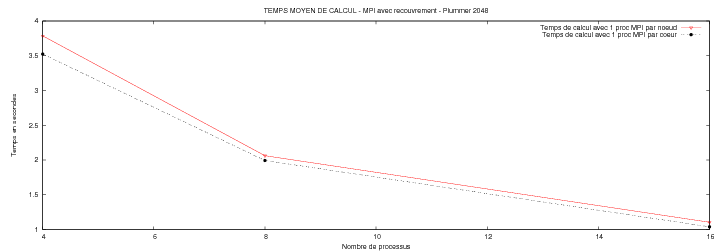
\includegraphics[angle=90]{perf_plumer2048bare2048_MPI.png}
  \caption{Temps total de calcul avec MPI}
  \label{fig:perf_plumer2048bare2048_MPI}
\end{figure}

\section{programme parallèle hybride MPI+OPEN\_MP}
La courbe de la figure \ref{fig:perf_plumer2048bare2048} représente les résultats obtenus après l'exécution de notre programme sur les corps du fichier baredisk\_2048-plummer\_2048.nemo avec MPI-openMP.

\begin{figure}[htbp]
  \centering
  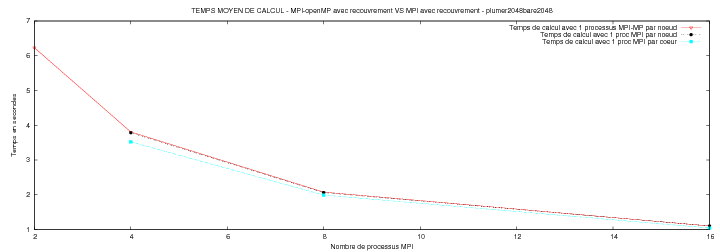
\includegraphics[angle=90]{perf_plumer2048bare2048.png}
 \caption{Temps total de calcul avec MPI couplé avec openMP}
\label{fig:perf_plumer2048bare2048}
\end{figure}



\chapter{Problèmes rencontrés }
\thispagestyle{fancy}
\par Le problème majeur de ce projet a été le petit nombre de salles à notre disposition 
pour effectuer nos tests et le nombre de machines actives dans chaque salle.
Nous ne disposions que d'une salle avec 16 machines. 

\par Le manque de pratique à mélanger MPI et OPEN\_MP a rendu notre programme 
hybride quelque peu hasardeux !!


\chapter{Conclusion}
\thispagestyle{fancy}
\input{chapter_6/conclusion}


\end{document}
